\documentclass[12pt,a4paper]{report}
\usepackage[spanish]{babel} % Corta palabras en español
\usepackage[utf8]{inputenc} % Escribir con acentos, ñ,
\usepackage{anysize} %para los márgenes
\usepackage{fancyhdr}
\pagestyle{fancy} %herramientas de encabezado
\usepackage{graphicx} % utilizar enlaces y poder insertar gráficos
\usepackage{indentfirst} %para identar despues de cada parrafo
%\usepackage{gensymb} %para añadir el símbolo de los grados celsius, etc
\usepackage{eurosym} %Paquete para introducir el símbolo del Euro
\usepackage[colorlinks=true,linkcolor=black,urlcolor=blue,pdftex]{hyperref} 
\usepackage{hyperref}
%\title{PROYECTO FINAL\\ DE \\CARRERA \\ ROCAMGO\\}
%\date{Version 1.0, \today}
\author{David Medina Velasco \and Víctor Ramírez de la Corte}

\fancyhead[R]{}
\fancyhead[C]{}
\fancyfoot[C]{\thepage}
%\fancyfoot[R]{David Medina Velasco \\ Víctor Ramírez de la Corte}
%fancyhdr --> paquete con bastantes herramientas para el encabezado y pie de página

\begin{document}
\part*{PROYECTO\\ FINAL\\ DE \\CARRERA \\ ROCAMGO\\}
%\maketitle

\marginsize{3cm}{2cm}{2cm}{2cm} % márgenes {izq}{der}{up}{down}.
\tableofcontents  %indice

 
\chapter*{Preambulo} 

Nos gustaría agradecer a: 
\begin{itemize} 
    \item Los compañeros de la asociación de software libre de Sevilla Sugus 
    GNU/Linux, los cuales nos han enseñado y ayudado mucho.  
    \item Los compañeros del club de go de Sevilla Ubicuo ki-in, los cuales nos
    han ofrecido lugar y materiales para probar el proyecto y siempre hemos 
    recibido su apoyo.  
    \item A D.Francisco Sivianes Castillo, nuestro tutor del proyecto, el cual 
    nos ha dedicado todo el tiempo que hemos requerido sin miramientos, 
    ayudandonos con nuestras dudas y guiandonos para la correcta finalización 
    del proyecto.  
    \item A D.Carlos Manuel Martin Cornejo, el cual ha colaborado con la 
    realización de la conexión con los servidores de go.  
    \item A Jaime Cornejo Pérez, por ayudarnos con el logo y comunicación con 
    los administradores del servidor de KGS.  
    \item A nuestros familiares, parejas y amigos.
\end{itemize}


\chapter{Conceptos}

\section{Software libre}

El software libre (en inglés free software, aunque esta denominación también se
confunde a veces con 'gratis' por la ambigüedad del término 'free' en el idioma
inglés) es la denominación del software que respeta la libertad de los usuarios
sobre su producto adquirido y, por tanto, una vez obtenido puede ser usado,
copiado, estudiado, modificado, y redistribuido libremente. Según la Free
Software Foundation, el software libre se refiere a la libertad de los usuarios
para ejecutar, copiar, distribuir, estudiar, modificar el software y
distribuirlo modificado.

El software libre suele estar disponible gratuitamente, o al precio de costo de
la distribución a través de otros medios; sin embargo no es obligatorio que sea
así, por lo tanto no hay que asociar software libre a 'software gratuito'
(denominado usualmente freeware), ya que, conservando su carácter de libre,
puede ser distribuido comercialmente ('software comercial'). Análogamente, el
'software gratis' o 'gratuito' incluye en ocasiones el código fuente; no
obstante, este tipo de software no es libre en el mismo sentido que el software
libre, a menos que se garanticen los derechos de modificación y redistribución
de dichas versiones modificadas del programa.

Tampoco debe confundirse software libre con 'software de dominio público'. Éste
último es aquel software que no requiere de licencia, pues sus derechos de
explotación son para toda la humanidad, porque pertenece a todos por igual.
Cualquiera puede hacer uso de él, siempre con fines legales y consignando su
autoría original. Este software sería aquel cuyo autor lo dona a la humanidad o
cuyos derechos de autor han expirado, tras un plazo contado desde la muerte de
este, habitualmente 70 años. Si un autor condiciona su uso bajo una licencia,
por muy débil que sea, ya no es del dominio público.


\section{¿Qué es el go?}

El go es un juego de mesa estratégico por turnos para dos jugadores. Es 
también conocido como igo (japonés), weiqi (chino) o baduk (coreano). El go 
es notable por ser rico en complejas estrategias a pesar de sus simples reglas.

El juego se realiza por dos jugadores que alternativamente colocan piedras
blancas y negras sobre las intersecciones libres de una cuadrícula de 19x19
líneas. El objetivo del juego es controlar una porción más grande del tablero
que el oponente. Una piedra o grupo de piedras se captura y retira del juego si
no tiene intersecciones vacías adyacentes, esto es, si se encuentra
completamente rodeada de piedras del color contrario.

Ubicar piedras juntas ayuda a protegerlas entre sí y evitar ser capturadas. Por
otro lado, colocarlas separadas hace que se tenga influencia sobre una mayor
porción del tablero. Parte de la dificultad estratégica del juego surge a la
hora de encontrar un equilibrio entre estas dos alternativas. Los jugadores
luchan tanto de manera ofensiva como defensiva y deben elegir entre tácticas de
urgencia y planes a largo plazo más estratégicos.

El go se originó en China hace más de 2 500 años y aunque no se sabe con
exactitud cuándo fue inventado, hacia el 300 a.C. era ya un pasatiempo popular,
como viene indicado en una referencia al juego en los Analectas de Confucio.
Restos arqueológicos muestran que este antiguo juego se jugaba en un tablero de
una cuadrícula de 17 x 17, pero en la época en la que el juego ya había llegado
a Corea y Japón, sobre el Siglo VII, los tableros habituales eran ya de 19 x 19.

El juego es muy popular en Asia Oriental, pero recientemente ha ganado cierta
popularidad en otras partes del mundo. El go llegó a Europa a través de Japón,
por ello es más conocido internacionalmente por su nombre japonés.


\section{¿Qué es un archivo .sgf?, para que sirve y como podemos abrirlo}

\label{sgf} Un archivo .sgf es un archivo donde se guarda una partida de
go. Como el formato es usado también para muchos juegos de tablero, está
bastante extendido y casi todos los programas de go lo soportan.

El archivo .sgf nos sirve para comentar una partida (como podemos ver en la
imagen) y hacer pruebas directamente desde un programa. Otro de los muchos
usos que tiene es guardar todas tus partidas para poder verlas en un futuro sin
ocupar apenas espacio en el disco. % TODO añadir imagen

Algunos programas que existen para abrir los .sgf pueden ser, por ejemplo,
quarry, qgo o CGoban. No solo sirven para abrir .sgf, suelen también servir para
jugar en servidores o contra una IA. % TODO comentar que no existe IA like ajed


\chapter{Objetivos} 

\section{Objetivos del proyecto} 

En los inicios de este proyecto, los objetivos que nos propusimos era poder
jugar una partida por Internet utilizando un tablero real, para ello
necesitaríamos un robot que nos pusiera las piedras del rival, una cámara para
capturar lo que está pasando en el tablero y un ordenador conectado a algún
servidor de go. Con todo hecho, el uso del programa no solo sería el de jugar
una partida en tablero físico, sino que también podríamos guardar una partida
completa observándola, y subirla en tiempo real a Internet, cosa que
agradeceríamos los jugadores de go, ya que el subir una partida de go por
streaming o subirla a mano, no es siempre posible, y este proyecto ayudaría la
facilidad de subir una partida sin tener que estar atento durante toda la
partida y sin necesitar una gran conexión a Internet, ya que con este sistema,
la información que enviamos al servidor es mínima. 

Si desarrollamos un poco más los objetivos, necesitaríamos un brazo robótico
rápido y preciso, una cámara que grabase videos con imágenes de una buena calidad, para evitar que saliesen borrosas,
con lo cual podríamos descartar cámaras VGA, y mucho tiempo y conocimientos de
programación, ya que el tratamiento de imágenes no es simple. 

Al investigar bastante sobre todos estos temas, nuestro objetivo cambió un poco
de cara a presentar el Proyecto Fin de Carrera, aunque en un futuro queremos
terminar nuestra idea inicial. Nuestro objetivo actual es subir una partidade go
que se esté jugando, para poder utilizar este proyecto en los torneos de go y
subir al menos la partida más interesante que se esté jugando en cada ronda. De
camino también guardamos la partida en un archivo .sgf [\ref{sgf}], para luego
poder modificarla con total libertad.

Para que el programa funcione correctamente, debemos tener una maquina con linux como sistema operativo, ya que pretendemos que nuestro programa funcione en cualquier dispositivo capaz de ejecutar este sistema operativo.   

Para ello, a nivel hardware necesitaremos solo una camara web grabando la partida que se este jugando y el tablero de go donde se jugará la partida.
No obstante, tambien podremos realizar nuestros objetivos tan solo teniendo 
un video de una partida.

%Imagen de la disposicion hardware correcta, que queremos que se use.

%\includegraphics[scale=0.08]{hardware.jpg}

Con este proyecto pretendemos conocer y mejorar nuestros conocimientos de 
herramientas y lenguajes de programación, así como de algunas librerías
interesantes, entre las cuales se encuentra OpenCv, librería sobre el
tratamiento de imágenes, el cual se encuentra actualmete en pleno auge. 

Al ser un proyecto donde trabajaremos más de una persona, entran en juego el
compañerismo, responsabilidad y comunicación. 

Los principales objetivos en este proyecto en su comienzo, era aprender:
\begin{itemize} 
    \item Python para el desarrollo del programa. 
    \item OpenCv para el tratamiento de imagenes. 
    \item Gtk para el entorno de ventanas del programa. 
    \item Unittest2 para el testeo del código. 
    \item Epydoc para la documentación del código. 
    \item Git para el control de versiones. 
    \item Redmine para gestión del proyecto. 
    \item Glade para el desarrollo visual de interface grafica con gtk.
    \item Latex para escribir la documentación. 
\end{itemize}


\chapter{Antecedentes y motivación}

La asistencia a unos cuantos de torneos de go, el amor por este maravilloso
juego y las ganas de aprender más y subir de nivel, nos hicieron pensar en crear
un programa para grabar nuestras propias partidas y poder jugar en un tablero
físico mediante Internet, ya que el jugar en un tablero físico motiva bastante
más que jugar por internet. Como aquí en España el juego todavía no está muy
extendido y no existen tantos Clubes como en Korea o en Japón, tenemos que
conformarnos la mayoría de las veces con jugar por Internet, lo cual pierde un
poco la esencia del juego, ese tacto de las piedras, el sonido de contacto de la
piedra en el tablero, y como no, el estar delante de tu oponente. 
En los torneos de go, existe una concentración al jugar que parece ser mayor que
la que normalmente tenemos, parece que jugamos mejor y pensamos un poco más nuestras
jugadas, por lo tanto, si tuvieramos la oportunidad de capturar estas partidas,
podríamos aprender mucho de ellas, tanto de los aciertos como de los errores. 
Estas partidas, actualmente se registran de dos formas: 
\begin{itemize}
    \item Utilizando el método antiguo, registrando la partida en un kifu. 
    \item Utilizando la tecnología, móviles, ordenadores, tablets, ...
\end{itemize} 

La partida puede registrarla alguno de los dos jugadores, lo cual puede
desconcentrar un poco al jugador, ya que no estará totalmente centrado en la
partida; o una persona ajena a la partida, la cual debe permanecer 1 o 2 horas
como mínimo delante del tablero apuntando todas esas jugadas. 

Como nota decimos que los jugadores que son muy fuertes, suelen acordarse de la
partida entera, pero al no ser este nuestro caso, ni el de otros muchos, nos
viene mejor una ayuda. 

\parskip 2ex
Todo esto nos llevó a pensar hacer este software, tanto para mejorar la forma de
registrar estas partidas para que todos podamos verla, como para poder grabar
nuestras propias partidas y poder ver nuestros errores una vez acabada, para así
mejorar. 


\chapter{Implementación}

\section{Herramientas utilizadas}


\subsection{Latex} 
% Explicacion
LaTeX es un sistema de composición de textos que está formado mayoritariamente 
por órdenes construidas a partir de comandos de TeX (lenguaje «de bajo nivel»,
en el sentido de que sus acciones últimas son muy elementales) pero con la 
ventaja añadida de poder aumentar las capacidades de LaTeX utilizando comandos 
propios del TeX descritos en The TeXbook. Esto es lo que convierte a LaTeX en 
una herramienta práctica y útil pues, a su facilidad de uso, se une toda la 
potencia de TeX. Estas características hicieron que LaTeX se extendiese 
rápidamente entre un amplio sector científico y técnico, hasta el punto de 
convertirse en uso obligado en comunicaciones y congresos, y requerido por 
determinadas revistas a la hora de entregar artículos académicos.
Su código abierto permitió que muchos usuarios realizasen nuevas utilidades que
extendiesen sus capacidades con objetivos muy variados, a veces ajenos a la
intención con la que fue creado: aparecieron diferentes dialectos de LaTeX que,
a veces, eran incompatibles entre sí. Para atajar este problema, en 1989 Lamport
y otros desarrolladores iniciaron el llamado «Proyecto LaTeX3». En el otoño
boreal de 1993 se anunció una reestandarización completa de LaTeX, mediante una
nueva versión que incluía la mayor parte de estas extensiones adicionales (como
la opción para escribir transparencias o la simbología de la American
Mathematical Society) con el objetivo de dar uniformidad al conjunto y evitar la
fragmentación entre versiones incompatibles de LaTeX 2.09. Actualmente cada año 
se ofrece una nueva versión, aunque las diferencias entre una y otra suelen ser 
muy pequeñas y siempre bien documentadas.
Con todo, además de todas las nuevas extensiones, la característica más
relevante de este esfuerzo de re-estandarización fue la arquitectura modular: se
estableció un núcleo central (el compilador) que mantiene las funcionalidades de
la versión anterior pero permite incrementar su potencia y versatilidad por
medio de diferentes paquetes que solo se cargan si son necesarios. De ese modo,
LaTeX dispone ahora de innumerables paquetes para todo tipo de objetivos, muchos
dentro de la distribución oficial, y otros realizados por terceros, en algunos
casos para usos especializados.

\parskip 2ex
Nosotros hemos utilizado Latex para la documentación, por que queda mucho más
bonita y nos vendría bien para aprender un poco. 


\subsection{TravisCI}

Como la integración continua aplicada al desarrollo distribuido está cogiendo
cada vez más fuerza, hemo aprovechado la herramienta de Travis CI, que es un
sistema distribuido de generación e integración continua libre.
Travis CI te permite conectar tu repositorio de Github y probar tus tests
después de cada push. Soporta múltiples lenguajes, entre los cuales se encuentra
python, que es el usado por nosotros.
Travis CI tiene otras ventajas que no hemos usado todavía, pero que no
descartamos utilizar en un futuro, que es que el entorno de integración continua
esta compuesto de multiples runtimes o data stores. De este modo, podemos probar
nuestras librerías o aplicaciones contra distintas configuraciones sin tener que
tenerlas instaladas localmente. Tienen varias maquinas virtuales preparadas para
cada combinación, allí puedes instalar MySQL o lo que necesites.
Lo podemos enganchar sencillamente con nuestro repositorio público de Github en
un par de pasos para darle acceso de lectura a nuestro código y definir los test
necesarios. Tanto la documentación, como las herramientas para terceros y la
guía de desarrolladores con la propia API de Travis CI están bastante bien
explicadas y detalladas. 

\parskip 2ex
Hemos utilizado esta herramienta para aprender y con la finalidad de que
comprobara todos nuestros test después de cada push al servidor, está bien para
saber como ha ido evolucionando nuestro proyecto. 

\subsection{Editores de texto: Geany, Gedit y Vim}

\textbf{''Geany''} es un editor de texto ligero basado en Scintilla con características
básicas de entorno de desarrollo integrado (IDE). Está disponible para distintos
sistemas operativos, como GNU/Linux, Mac OS X, BSD, Solaris y Microsoft Windows.
Es distribuido como software libre bajo la Licencia Pública General de GNU.

\parskip 2ex
Nostros empezamos a utilizar este editor ya que nos facilitaba el autocompletado
y era bastante liviano, tenía coloreado de sintaxis y permitía la programación
con el lenguaje usado por nosotros, Python. 

\parskip 2ex

\textbf{''Gedit''} es un editor de textos compatible con UTF-8 para GNU/Linux,
Mac OS X y Microsoft Windows. Diseñado como un editor de textos de propósito
general, gedit enfatiza la simplicidad y facilidad de uso. Incluye herramientas
para la edición de código fuente y textos estructurados, como lenguajes de
marcado. Distribuido bajo las condiciones de la licencia GPL, gedit es software
libre. 

\parskip 2ex
Nosotros cambiamos a este editor por que aún era más simple y liviano que Geany,
y aunque no nos daba un buen autocompletado, tenía todo lo que queríamos,
coloreado de sintáxis, facilidad de uso, y también hay que tener en cuenta que
es el editor por defecto del entorno de escritorio GNOME, el cual hemos
utilizado bastante. 

\parskip 2ex

\textbf{''Vim''} es un editor hecho por programadores para programadores. Para
facilitar la programación, Vim dispone de un modo 'editar, compilar, corregir'.
De la misma forma que los entornos de desarrollo integrados, puede editar el
código fuente además llamar a un compilador externo, e interpretar sus
resultados. Si hay errores de compilación, éstos se muestran en una ventana. Los
mensajes de error dirigen al usuario a la zona en la que se han encontrado para
poder así corregirlos. Entonces vuelve a empezar el ciclo "editar, compilar,
corregir" y, si es necesario, corregir nuevos errores. El trabajo del
programador también se ve facilitado por el resaltado de sintaxis y la
funcionalidad de plegado de código.

\parskip 2ex Empezamos a utilizar este editor ya que está preparado para
programadores, y su filosofía se basa es hacerlo todo con el mínimo número de
pulsaciones de teclado, lo cual, cuando nos acostumbremos a utilizarlo,
conseguiremos una gran mejora de productividad. También decir que Vim es el
programa que actualmente más plugins tiene, y es altamente configurable, para
adecuarse al perfil de cada programador, cosa que nos ha gustado muchísimo. 


\subsection{Controladores de versiones: Subversion y Git}

\textbf{''Subversion''} es un sistema de control de versiones centralizado diseñado
específicamente para reemplazar a CVS. Es software libre bajo una licencia de
tipo Apache/BSD y se le conoce también como svn por ser el nombre de la
herramienta utilizada en la línea de comando.  Una característica importante de
Subversion es que, a diferencia de CVS, los demas archivos con versionamiento no
tienen cada uno un número de revisión independiente, en cambio, todo el
repositorio tiene un único número de versión que identifica un estado común de
todos los archivos del repositorio en un instante determinado del repositoro que
se esta trabajando. Subversion puede acceder al repositorio a través de redes,
lo que le permite ser usado por personas que se encuentran en distintas
computadoras. A cierto nivel, la posibilidad de que varias personas puedan
modificar y administrar el mismo conjunto de datos desde sus respectivas
ubicaciones fomenta la colaboración. Se puede progresar más rápidamente sin un
único conducto por el cual deban pasar todas las modificaciones. Y puesto que el
trabajo se encuentra bajo el control de versiones, no hay razón para temer por
que la calidad del mismo vaya a verse afectada, si se ha hecho un cambio
incorrecto a los datos, simplemente deshaga ese cambio. 

\parskip 2ex Subversion ya lo habíamos utilizado anteriormente, y es una
herramienta que nos parece bastante buena, sobre todo por que al ser dos
personas, nos facilitaba mucho el trabajo, y para las cosas básicas, es bastane
fácil de utilizar. 

\parskip 2ex

\textbf{''Git''} es un software de control de versiones distribuido diseñado por
Linus Torvalds, pensando en la eficiencia y la confiabilidad del mantenimiento
de versiones de aplicaciones cuando estas tienen un gran número de archivos de
código fuente. Al principio, Git se pensó como un motor de bajo nivel sobre el
cual otros pudieran escribir la interfaz de usuario o front end. Sin embargo,
Git se ha convertido desde entonces en un sistema de control de versiones con
funcionalidad plena. Hay algunos proyectos de mucha relevancia que ya usan Git,
en particular, el grupo de programación del kernel de Linux. 

\parskip 2ex 
Git no lo habíamos utilizado nunca, pero teníamos ganas de aprender y empezamos
a usarla. Esta herramienta nos ha dado un poco de dolores de cabeza, pero
finalmente nos está gustando y le estamos viendo bastante ventajas respecto a
Subversion. 


\subsection{Servidores de Go: IGS y KGS} %TODO añadir otros que hay, LLGS 

\textbf{''El servidor IGS''} nos ofrece un gran lugar para jugar, ver, estudiar
y disfrutar del juego de Go en Internet. Podemos encontrar cientos de jugadores
de dintintas partes del mundo y diferentes nivelesde juego, desde principiantes
hasta profesionales. 

\parskip 2ex
Ademas este servidor ofrece un protocolo de comunicaciones abierto y muy bien
documentado, el cual hemos utilizado para subir la partida mientras se va
jugando. 

\parskip 2ex

\textbf{''KGS Go Server''}, llamado comunmente KGS, es un servidor de Go popular
al cual podemos acceder desde http://www.gokgs.com/. Normalmente hay más de 1500
personas conectadas en cualquier momento, por lo que es uno de los servidores
más grandes en el mundo. Muchas de las partidas de perfil alto de los torneos se
retransmiten en KGS. KGS abrió por primera vez bajo el nombre Igoweb en abril
de 2000.  Apenas un mes después, el autor hizo un acuerdo con Kiseido y fue
rebautizado con el Kiseido Go Server. Su nombre se cambió a KGS Go Server en
2006. William M. Shubert es el desarrollador de KGS. El cliente conocido como
CGoban3 ha sido escrito en Inglés, y ha sido traducido a muchos idiomas
diferentes, como japonés, francés, italiano, alemán, chino y español entre
otros. 

\parskip 2ex
Nosotros también hemos intentado subir la partida a este servidor, pero el
protocolo de comunicación que se usa no es software libre, por lo tanto no
tenemos acceso a él para subir una partida fácilmente, ya que no hemos
encontrado tampoco mucha comunicación. En estos momentos estamos intercambiando
correos con el desarrollador de KGS y algunos administradores para ver si
podemos hacer algo y que se permitan subir partidas a este servidor tan
conocido. 


\subsection{Sistemas Operativos: Debian y Linux Mint}

\textbf{''Debian''} es un sistema operativo libre, desarrollado por más de mil
voluntarios alrededor del mundo, que colaboran a través de Internet.  La
dedicación de Debian al software libre, su base de voluntarios, su naturaleza no
comercial y su modelo de desarrollo abierto la distingue de otras distribuciones
del sistema operativo GNU. Todos estos aspectos y más se recogen en el llamado
Contrato Social de Debian.  Nació en el año 1993, de la mano del proyecto
Debian, con la idea de crear un sistema GNU usando Linux como núcleo ya que el
proyecto Debian, organización responsable de su mantenimiento en la actualidad,
también desarrolla sistemas GNU basados en otros núcleos (Debian GNU/Hurd,
Debian GNU/NetBSD y Debian GNU/kFreeBSD).  Uno de sus principales objetivos es
separar en sus versiones el software libre del software no libre. El modelo de
desarrollo es independiente a empresas, creado por los propios usuarios, sin
depender de ninguna manera de necesidades comerciales. Debian no vende
directamente su software, lo pone a disposición de cualquiera en Internet,
aunque sí permite a personas o empresas distribuir comercialmente este software
mientras se respete su licencia.  Debian Linux puede instalarse utilizando
distintos mecanismos de instalación, como DVD, CD, Blu-Ray, memorias USB y
diskettes, e incluso directamente desde la red.

\parskip 2ex

\textbf{''Linux Mint''} es una distribución del sistema operativo GNU/Linux, basado en la
distribución Ubuntu (que a su vez está basada en Debian). A partir del 7 de
septiembre de 2010 también está disponible una edición basada en Debian.  Linux
Mint mantiene un inventario actualizado, un sistema operativo estable para el
usuario medio, con un fuerte énfasis en la usabilidad y facilidad de
instalación. Es reconocido por ser fácil de usar, especialmente para los
usuarios sin experiencia previa en Linux.  Linux Mint se compone de muchos
paquetes de software, los cuales se distribuyen la mayor parte bajo una licencia
de software libre. La principal licencia utilizada es la GNU General Public
License (GNU GPL) que, junto con la GNU Lesser General Public License (GNU
LGPL), declara explícitamente que los usuarios tienen libertad para ejecutar,
copiar, distribuir, estudiar, cambiar, desarrollar y mejorar el software. Linux
Mint es financiada por su comunidad de usuarios. Los usuarios individuales y
empresas que utilizan el sistema operativo pueden actuar como donantes,
patrocinadores y socios de la distribución. El apoyo financiero de la comunidad
y la publicidad en el sitio web ayuda a mantener Linux Mint libre y abierta.

\parskip 2ex
Como puede observarse, hemos intentado utilizar todas las herramientas libres
que hemos podido, incluyendo, como no, el sistema operativo. Como cada uno
tenemos nuestros gustos, cada uno de nosotros hemos utilizados el sitema
operativo que más se adecuaba a nuestros gustos. 


\subsection{Entornos de escritorio: Awesome y Cinnamon}

\textbf{''Awesome''} es un gestor de ventanas para X Window System desarrollado
en C y lenguaje de programación Lua. Este último también se utiliza para
configurar y ampliar el gestor de ventanas. Al igual que muchos gestores de
ventanas del tipo tiling window manager (tipo mosaico), hace lo posible para que
el usuario pueda manejar productivamente las ventanas sin el uso del ratón.  El
programa se incorpora en los repositorios de Debian GNU/Linux desde la versión
lenny en su versión 2. La nueva versión, 3.4.2 For The Restless, se encuentra en
los repositorios de Ubuntu y en la versión estable de Debian.

\parskip 2ex

\textbf{''Cinnamon''} es una bifurcación de GNOME Shell, desarrollado
inicialmente por Linux Mint. Intenta proveer un entorno de escritorio más
tradicional basado en la metáfora de escritorio, como GNOME 2. Cinnamon usa
Muffin, una bifurcación del gestor de ventanas de GNOME 3 Mutter, como su gestor
de ventanas desde la versión 1.2.

\parskip 2ex
Al igual que con el sistema operativo ha ocurrido con el entorno de escritorio,
gracias a que en la comunidad del Software Libre se ofrecen inifinidad de
posibilidades de entornos, cada uno hemos utilizado el que más nos gustaba.

\section {Implementación del proyecto}

Como todo proyecto, la implementacion la hemos dividido en funcionalidades que
queriamos que tuviese el proyecto. Las principales funcionalidades, que a su vez
las hemos dividido para hacer un codigo mas legible y modular, son:
\begin{itemize} 
    \item Detección de cámara.
    \item Detección de tablero.
    \item Detección de movimiento del tablero.
    \item Idealización del tablero.
    \item Detección de piedras.
    \item Comunicación con el servidor. Transmisión de partida por Internet.
\end{itemize}

La realización de este proyecto a supuesto muchísimos cambios en las
implementaciones, ya que hemos tenido que desechar muchas de ellas por motivos
diferentes que nos hemos ido encontrando. 


\subsection{Detección de la cámara} 
Funcionalidad que nos busca y nos selecciona la cámara que queramos usar,
siempre y cuando exista alguna en nuestro ordenador. 

\paragraph{1ª Implementación: detección de cámaras solo en Linux}

Nuestra primera detección de cámaras solo estaba preparada para funcionar en
Linux, ya que utilizábamos una manera que solo funcionaba en Linux, y la cual,
si enchufabas y desenchufabas alguna cámara anteriormente, daba fallos, ya que
capturábamos las cámaras utilizando el dispositivo de video que se encontraban
en las direcciones /dev/videoX, siendo X el número de la cámara. 

\paragraph{2ª Implmentación: detección de cámaras utilizando opencv}

Esta implementación funciona bastante bien, ya que no solo funciona en Linux, 
si no que debería de funcionar en cualquier sistema operativo. También decir que
es una forma mejorada de detectar las cámaras, ya que no hay problemas si hemos
enchufado y desenchufado cámaras anteriormente. 


\subsection{Detección del tablero} 
Funcionalidad para la detección del tablero, ya sea de las intersecciones o de
las esquinas, para luego poder ubicar la posición de las piedras de alguna
manera. 

\paragraph{1ª Implementación: detección mediante líneas}
En este intento de implementación intentamos buscar las lineas del trablero 
mediante el tratamiento de imágenes y la función HoughLines de opencv, para 
luego buscar las intersecciones del tablero y así tener el tablero detectado. 
Pensamos que el tratamiento de esas líneas sería sencillo de procesar, pero al
existir tantas líneas y tener que buscar tantas intersecciones, se convertía en
una auténtica locura que no fuimos capaces de abordar, por lo tanto desechamos
esta implementación. 

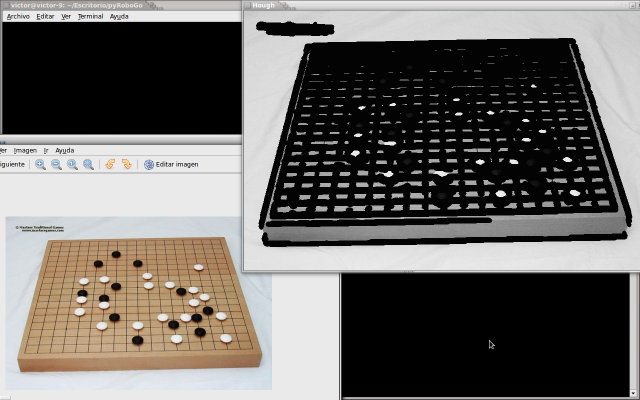
\includegraphics[scale=0.6]{detect-lineas.png}


Otro de los problemas era que el tablero estaría casi siempre con un poco de
perspectiva, y entonces no sabríamos que lineas escoger, ya que el tablero, al
ser de madera contiene muchas betas y podría detectar bastantes lineas que no
serían las buscadas. 
Más adelante nos dimos cuenta de que existe otro problema con esta
implementación, y es que cuando haya piedras encima del tablero, habrá bastante
problemas. 
 

\paragraph{2ª Implementacion: detección mediante intersecciones}

Despues de entender que la forma anterior de buscar el tablero no era efectiva,
decidimos ponernos a trabajar en otra idea. Esta vez decidimos hacerlo, atacando
a las intersecciones, usando templates. Esta forma consiste en buscar en la
imagen que recibimos de la cámara el template de una interseccion (imagen
que contine solo la interseccion). Con esto conseguíamos detectar casi a la
perfección casi todas las intersecciones, y las que no sacábamos podíamos
sacarlas mediante una malla. 

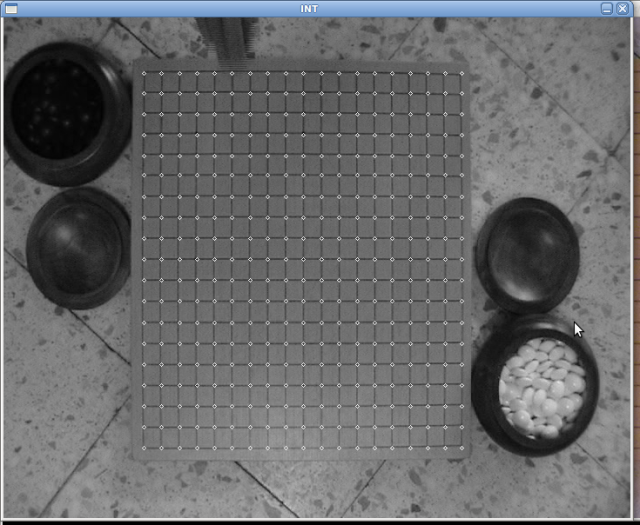
\includegraphics[scale=0.6]{detec-intersecciones.png}

El problema de todo esto era el coste de ejecución que conllevaba hacerlo, a
parte, también nos topábamos con el problema de que necesitábamos un tablero que
tuviese la mínima perspectiva posible, ya que si no el template no lo pillaría. 
Como pasa con la anterior implementación, otro problema es que cuando se empieza
a jugar la partida, estas intersecciones se tapan. 


\paragraph{3ª Implementación: Haartraining, aprendizaje}

Tras dos intentos fallidos, comenzamos a estudiar la siguiente idea, sacada de
distintos programas de camaras de fotos, los cuales detectan y recuadran la
cara. Esta forma de hacerlo se llama HaarTraining, y consiste en enseñarle al
ordenador a buscar un tablero, introduciendo en un programa de aprendizaje
imagenes donde estén los tableros, indicandole la posicion. En ese proceso de
aprendizaje tambien hay que enseñarle fotos que no contengan el tablero.
Después de estudiarlo, nos dimos cuenta de varias cosas que hicieron que no
continuásemos por este camino. La primera de ellas es el tiempo dedicado a la
realización de las fotos y posterior análisis manual, para indicar el lugar del
tablero. La segunda el tiempo de ejecucion del aprendizaje, suele llevar unas
dos semanas, en un ordenador potente. Y por último, la tercea y más importante,
es que despues de las dos primeras, nadie te aseguraba con una minima certeza 
que esta posibilidad fuese a funcionar.

En la siguiente imagen podemos ver un claro ejemplo que usan las camaras de foto
con este tipo de implementacion.

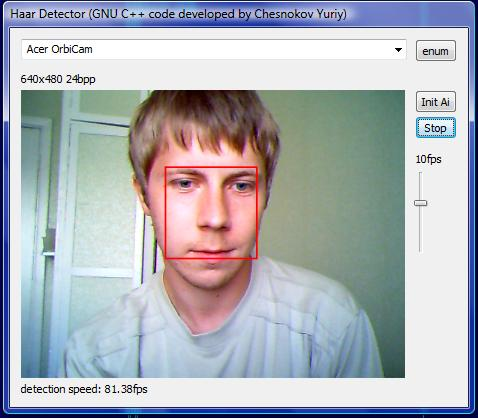
\includegraphics[scale=1]{haartraining.jpg} 

Estuvimos bastante tiempo investigando y probamos con 40-50 imágenes, en vez de
con 3000 como mínimo, que es lo que piden, y como esperábamos, fue un fracaso,
no encontraba tablero ninguno con tan pocas imágenes de aprendizaje. 

\paragraph{4ª Implementación: detección mediante contornos}

Finalmente y tras tres intentos fallidos, decidimos hacerlo buscando contornos.
Gracias a una funcion de openCv conseguimos encontrar la forma que menos fallos
nos ha dado, cumple con los requisitos y soluciona casi todos los problemas.
Esta funcion devuelve contornos, por ello uno de los requisitos que debemos
pedir para la correcta ejecución de este programa es que el fondo donde se
coloque el tablero, sea lo más liso posible, cosa que podemos conseguir con
facilidad utilizando un mantel o hule, aunque no es totalmente necesario, pero
facilita y ayuda al mejor funcionamiento del programa. Debido a la gran cantidad
de test que ha pasado correctamente esta implementacion y dado que los test que
han fallado son debido a la mala calidad de las imágenes (sobre todo a causa de
la luminosidad de las imágenes), hemos considerado que es la correcta. Además,
perdemos el problema de la perspectiva, pues lo que detectamos es el contorno.


\subsection{Detección de movimiento del tablero}

Tenemos que comentar que esta implementación fue un poco tardía, ya que nosotros
suponíamos que el tablero no se movería, pero en casi todas las partidas de
torneo, inconscientemente, para tener una mejor perspectiva del tablero o
acercarlo, el tablero se mueve durante la partida. Así que al encontrarnos con
este problema, nos dimos cuenta de que las implementaciones del tablero que
hicimos al principio, no nos servían. 

\paragraph{1ª Implementación: detección de cambios en los bordes del tablero}

En principio, para detectar si el tablero se movía o no, buscamos que existieran
cambios en los bordes del tablero, ya que si los movemos, estos deben de
cambiar. Al ver que cada vez que metíamos la mano para poner una piedra,
empezaba a cogerlo como cambio, o el hecho de que cambiara la luz un poco, daba
movimiento del tablero, descartamos esta opción. 

\paragraph{2ª Implementación: cambio de esquinas detectados} 

Esta segunda implementación nos pareció impensable la primera vez, ya que lo que
hacemos es detectar contornos durante todo el tiempo, y cada vez que los
encuentre, busque si son los mismos que los que ya teníamos o han variado. Si
han variado, para decidir si ha pillado bien las esquinas o no, utilizamos una
serie de reglas matemáticas. 
Quizás el que tardara tanto en detectar el tablero con las implementaciones
anteriores, no nos hizo pensar en esta forma de hacerlo, pero al ver que es
factible con los contornos, hemos utilizado esta forma, y no parece ir mal del
todo, aunque no está asegurado que permaneca tal y como está, si es probable que
sea parecido. 

\subsection{Idealización del tablero} 

Una vez detectado el tablero correctamente y antes de ponernos a buscar piedras
por toda la imagen, llegamos a la conclusion que seria mas conveniente conseguir
el tablero en un modelo ideal, como si las imágenes que recibimos fuesen tomadas
como nosotros las queremos, que es desde arriba, sin perspectivas.  Gracias a
opencv conseguimos con la funcion WarpPerspective y GetPerspectiveTransform que 
la imagen se ponga con una
perspectiva perfecta, recortando las partes de la imagen donde no está el
tablero, haciendo asi que la búsqueda de piedras sea una labor mucho más
sencilla. Para conseguir que esta función nos sirva, tuvimos que hacer un
testeo bastante amplio, pues las imágenes necesitan ser tratadas anteriormente
para el correcto funcionamiento de dicha funcion, con filtros como Canny y
Smooth, para detectar bordes o suavizar la imagen. 

\subsection{Deteccion de piedras} 

Una vez detectado el tablero correctamente,
pensabamos que la deteccion de piedras iba a ser mucho mas facil, aun asi, la
detección de piedras tambien ha pasado por un ciclo evolutivo de modificaciones
hasta madurar lo suficiente la idea, para conseguir finalmente un programa que
funcione tal y como teniamos pensado desde un primer momento. En un principio
nos pusimos manos a la obra con la búsqueda de piedras con las diferentes
implementaciones que os presentamos a continuación.
También debemos recordar, que la detección de
piedras, no es solamente detectar donde está cada piedra, también debemos
detectar el orden correcto en el que han sido colocadas y el color de la piedra,
tenemos que tener en cuenta que también existe la posibilidad de que una piedra
se retire del tablero. 

\paragraph{1ª implementación: detección de piedras por turnos}
En los inicios del programa, las piedras se detectaban de una forma poco
ortodoxa, pues en gran parte, los jugadores debian decirnos cuando terminaban su
turno, para asi tomar la foto en el momento justo, y poder analizarla
correctamente.  La forma de la busqueda de la piedra se hacia por diferencia de
imagenes, asi, cada vez que un jugador nos indicaba mediante un boton que habia
terminado el turno, captabamos una imagen y la comparabamos con la anterior, la
funcion "diff" de OpenCv nos devuelve marcadas las diferencias, que este caso
serian las piedras, despues dentro de esta imagen, buscamos circulos y
conseguiamos encontrar las piedras.  

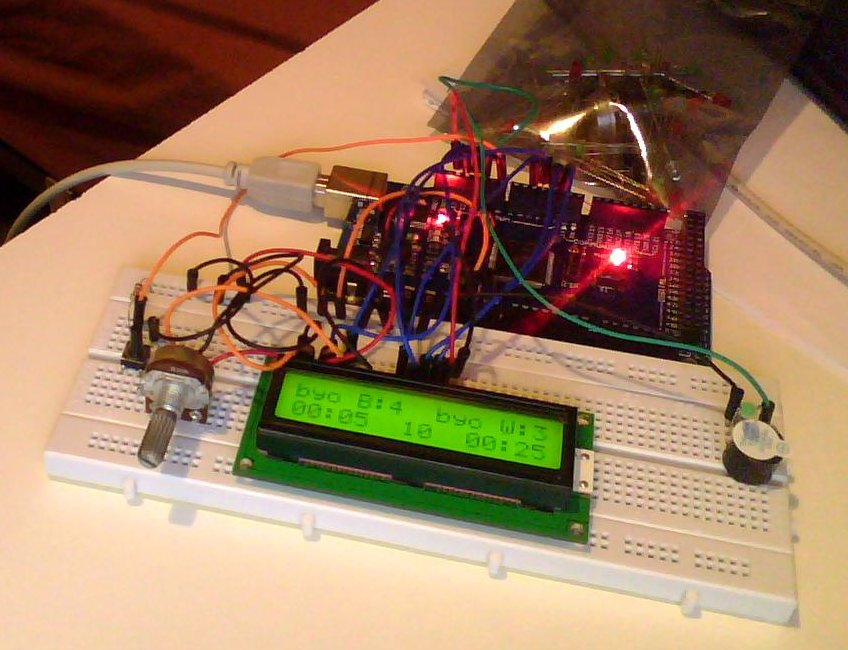
\includegraphics[scale=0.4]{reloj.jpg}

Esta forma fue eliminada al poco tiempo,pues una de nuestras ideas, es que el
jugador no tenga que preocuparse del programa, pues esta concentrado jugando.
Ademas, los factores externos eran demasiados, pues pensamos en modificar los
relojes de tiempo, para que el propio
boton que indicaba al reloj el final del tiempo, fuese el mismo que nos indicase
a nosotros el momento de tomar la foto. Con todo esto, lo unico que podiamos
conseguir es que nuestro programa no fuese funcional, ya que nadie podria hacer
uso de nuestro programa sin dicho reloj. Tras pensar distintas formas de
solucionar los problemas que daba dicha implementacion, decidimos cambiar por
completo la idea.  % TODO poner una explicacion del problema del joseki


\paragraph{2ª Implementación: detección por diferencias sin turnos}
En esta segunda implementación pensamos en suprimir el uso de botones y
decidimos buscar la diferencia de cada imagen con la anteior, buscando circulos
en esa diferencia. Esta solución nos pareció mucho mejor que la anterior, pero
empezamos a darnos cuenta que detectaba toda la trayectoria que hacia la piedra
hasta estar colocada en su sitio, haciendo que el programa nos detectase piedras
donde realmente no se habian puesto, esto se podria haber solucionado
estadísticamente, pero esto lo descubrimos más tarde, asi que en ese momento se
descartó esta idea y enfocamos la solución de otra forma. Además, el hacer la
diferencia de todas las imágenes conllevaba un coste de procesamiento a tener en
cuenta, al cual había que añadirle la búsqueda de círculos, suma que es
demasiado elevada y creaba un tiempo de retreso que se iba acumulando, haciendo
que en determinado momento fallase el programa.

\paragraph{3ª Implementación: detección por circuferencias y estadística}
Y como dice el refrán, a la tercera va la vencida. Esta vez, ya teniamos más
experiencia y el tablero ya estaba idealizado. Por esto, pensamos que la mejor
solución podría ser la más sencilla, para ello, sin hacer tratamiento ni
diferencias, buscamos círculos en la imagen ideal. Con una matriz de estadística
temporal, vamos buscando si los círculos se quedan de forma estable en una
posición, y en tal caso, podemos asegurar que la piedra esta colocada en ese
lugar, esta solución, ademas permite llevar bien la cuenta de los turnos y el
momento en el que se puso la piedra, pues aunque tenga que pasar un tiempo para
asegurar que está la piedra, sabemos el momento en el que se puso. Ademas el
coste de ejecución es asumible.

\paragraph{Buscando colores}
%variar una variable. Cambiar el umbral de brillo
% meter dentro de la búsqueda de piedras mejor

Como en cada parte del proyecto, esta tambien ha tenido su evolucion desde que
empezamos a plantearlo hasta el resultado final, mucho mas pulido y funcional.
En un principio y dado que los jugadores nos iban a ir marcando el ritmo de
turnos, simplemnte debiamos saber si le tocaba colocar a blancas o negras, como
siempre empiezan negras, por reglas del propio juego, solo debiamos detectar la
piedra que se colocaba y automaticamente teniamos el color.  Debido a que esto
cambio a lo largo del tiempo y en la actualidad la forma de encontrar piedras es
distinta, debemos saber de que color es la piedra que se ha detectado en cada
momento, para ello una vez que detectamos una piedra, debemos asegurarnos de que
color es. La forma de hacerlo es buscando en el punto central donde esta situada
la piedra e ir a su pixel y analizar el color. Gracias a openCv esta labor es
relativamente sencilla, pero nos dimos cuenta, debido a la calidad de las
imagenes, que no todo iba a ser color de rosa. El gran problema que tenemos es
que las piedras al ser redondeadas, la camara capta reflejos de dichas piedras
haciendo que el color de las piedras pueda llegar a confundirse facilmente si no
cogen un numero amplio de muestras para saber el color. Aun asi, los test dan
fallos a veces, para evitar esto, hay que variar una variable, siendo este uno
de los puntos a seguir trabajando en un futuro en nuestro programa.


\subsection{Conexion con el servidor}

Para la conexion al servidor comenzamos intentandolo con los servidores de KGS,
pero la falta de documentacion de protocolos de dicho servidor y el tener un
protocolo cerrado hizo imposible esta tarea. Aun asi, queremos hacer posible la
conexion a este servidor, pues es de los mas usados. Actualmente el programa se
conecta a IGS a traves de un usuario registrado siguiendo el protocolo de dicho
servidorl, que es libre.


\chapter{Manual de usuario}

\section{Guia de instalación} 

Para la instalación del proyecto, al menos de lo que se encuentra activo
actualmente, porque como hemos comentado, el proyecto no está terminado, pero
podremos ver los últimos cambios utilizando la última versión disponible en
GitHub del proyecto. Este proyecto se ha probado solamente en Linux, aunque
debería de funcionar en otros Sistemas operativos, ya que se ha realizado la
programación pensando en ello. 
La guía de instalación la haremos pensado en que se tiene un entorno Linux, que
es donde únicamente podemos afirmar que funciona el proyecto. Comenzamos
descargándonos el proyecto desde GitHub, para ello necesitaremos tener instalado
git, que en las distribuciones de Linux basadas en debian, podemos instalarlo de
la siguiente manera: 

% TODO comando
\begin{verbatim}
sudo apt-get install git
\end{verbatim}

Ejecutamos el siguiente comando para descargarnos el proyecto: 

\begin{verbatim}
git clone git@github.com:Virako/Rocamgo.git
\end{verbatim}

Dentro de esta carpeta nos encontraremos con los últimos cambios realizados en
el proyecto. Para hacerlo funcionar deberemos ejecutar desde la carpeta raiz,
que se llamará Rocamgo si no se ha cambiado, el siguiente comando:

\begin{verbatim}
python src/rocamgo.py
\end{verbatim}

En estos momentos, las versión que se encuentra en el repositorio, para hacer
las pruebas no utilizamos cámaras, sino que utilizamos un video, que es con lo
que hacemos las pruebas. Como el video al cual le hacemos las pruebas ocupa 3GB,
este archivo no lo adjuntamos, hay que pedírselo a los desarroladores. 

Si queremos utilizar la cámara para hacer la prueba, deberemos de
comentar/descomentar unas líneas del archivo rocamgo.py, que se encuentra dentro
de src. Quedando la parte a cambiar de la siguiente manera: % TODO more code xD

\begin{verbatim}
def main():
    # Select camera from computer
    cam = Cameras()
    cams_found = cam.check_cameras()
    camera = cam.show_and_select_camera(); threshold=190
    #camera = CaptureFromFile('prueba2.avi'); threshold=150 # Test videos
    prev_corners = None
    current_corners = None
    good_corners = None
    ideal_img = None
    goban = Goban(GOBAN_SIZE)

    while camera: 
        # Select image from camera 
        img = camera.get_frame()
        #img = QueryFrame(camera) # Test videos
\end{verbatim}

Para que funcione el proyecto, necesitaremos instalar unas cuantas de librerías
que hemos usado: opencv, unittest, nosetest, numpy, 

Para su instalacion, al igual que para instalar git, ejecutamos lo siguiente:

\begin{verbatim}
sudo apt-get install python-unittest2 python-opencv python-nose python-numpy
\end{verbatim}

Con todo esto, ya deberíamos de poder ejecutar el proyecto y que este funcione
correctamente. En el caso de que exista algún error, contactar con los
desarroles del proyecto. 


\section{Como utilizarlo}

Antes de empezar, debemos asegurarnos que tenemos preparado el terreno de juego, para ello necesitamos que el tablero este colocado en una superficie lo mas lisa posible y una camara web conectada al PC donde se ejecutará el programa, a poder ser de una buena calidad, apuntando al tablero donde se jugará la partida. Debemos intentar que la camara enfoque correctamente al tablero, centrando este dentro de la imagen lo maximo posible. El programa será capaz de funcionar siempre y cuando en la imagen se vean correctamente todas las partes del tablero.

Al ejecutar este proyecto, lo primero que te pedirá si está en modo captura de
video, será un usuario y una contraseña, los cuales son un usuario del servidor
IGS, el cual podemos crearnos en la página 
\url{http://www.pandanet-igs.com/igs_users/register}
Este usuario se pide para subir la partida a internet mientras se está
detectando. 

En el caso de que hayamos escogido la opción de detectar el tablero con la
cámara, la primera ventana será la selección de cámara en el caso de que existan
más de una, si solo existe una, esta la cogerá por defecto. Para seleccionar la
cámara que deseemos, pulsamos doble click encima de la cámara deseada.  Tras
seleccionar la cámara, pedirá el usuario y la contraseña, como en el caso
anterior. 


\section{Actualizaciones}

Para actualizaciones del proyecto, una vez lo hayamos descargado con git, solo
tenemos que entrar dentro del directorio y ejecutar git pull, el cual se
descargará los últimos cambios que haya en el servidor. 


\chapter{Conclusiones}

Desde el principio de este proyecto, hemos estado aprendiendo bastante sobre las
librerías de opencv, las cuales son una maravilla y nos han ayudado muchísimo en
la implementación de este proyecto. Creemos que todavía nos queda mucho que
aprender sobre estas librerías, las cuales esperamos aprender más en un futuro. 

Cuando nos hemos ido adentrando en el proyecto, nos han ido surgiéndo muchísimos
problemas, sobre todo con la detección del tablero, ya que lo pensado y la
realidad, se han ido distanciando un poco. 

La utilización de git nos ha hecho aprender y abrirnos la mente al utilizar un
controlador de versiones distribuidos, a parte de servirnos de mucha ayuda al
ser un proyecto en grupo. 

La gran utilización de python nos ha hecho subir nuestro nivel de programación
en este lenguaje.

El usar filosofía TDD y hacer test en el proyecto nos han ayudado a realizar
algunas cosas más rápido y comprobar el correcto funcionamiento de algunas
funcionalidades, como por ejemplo, en la detección del tablero. Gracias a esto
conocimos también algunas herramientas como TravisCI, la cual puede sernos de
gran utilidad más adelante. 

La utilización de Latex, al estar acostumbrados a programar, no nos ha resultado
muy complicada. Cuando observamos como quedan los documentos, la verdad es que
nos ha fascinado, y tenemos pensamiento de utilizarlo para otros textos en un
futuro, es una herramienta que nos ha cautivado.

El conectarnos al servidor de IGS, nos ha hecho que aprendamos a utilizar un
poco los sockets.

Aunque finalmente no utilizamos arduino para los relojes, también nos llevamos
un tiempo manejandolos y aprendimos bastante, ya que usamos botones, pantalla
LCD, potenciómetros y buzzer.

Destacar a vim dentro de todos los editores de texto que hemos utilizado, ya que
aunque la curva de aprendizaje sea bastante dura, finalmente podemos decir que
la productividad aumenta. 

Agradecer a toda la comunidad del software libre de nuevo, por que gracias a
ella, hemos tenido un sistema operativo con un software bastante bueno para la
realización de todo el proyecto, así como el acceso a una gran cantidad de
código libre para ver ejemplos de como hacer las cosas, ya que creemos que la
mejor forma de aprender es con ejemplos. Sin dejar atrás las webs de preguntas y
respuestas, los foros y los chats, que nos han solucionado más de una duda. 





\chapter{Lineas futuras}

El futuro de este proyecto sigue día a día, y esperamos que poco a poco se vaya
mejorando hasta conseguir todos los objetivos deseados, aunque por temas de
tiempo o dinero, no hemos podido terminar para este Proyecto Fin de Carrera. 

Principalmente queremos seguir mejorando la detección de partida de cara al
siguiente torneo de go, para ver si podemos llegar a utilizarlo completamente
para una partida real, en la cual seguramente aprendamos mucho y encontremos
errores nuevos para poder mejorar, por que como ya nos hemos dado cuenta, la
realidad se aleja de lo pensado, cada sitio donde se situe el tablero o que
cámara se escoja, seguramente de nuevos fallos que tendremos que ir puliendo
poco a poco. Estamos deseando llevar el proyecto al siguiente torneo para ver si
le gusta a la gente y ver su funcionamento en distintos sitios, con distinta
luminosidad, distintos jugadores que mueban más o menos el tablero, se usen
tableros o piedras distintas, en tonalidad sobre todo. 

Otra de las cosas que ya decidimos a mitad del proyecto de descartar, es hacer
el brazo robótico, porque un brazo rápido y preciso costaba muy caro, en precio
o en tiempo. En un futuro tenemos pensado gastarnos ese dinero o tiempo para
crear el brazo, ya que es una cosa que nos entusiasma bastante. Las
funcionalidades que aportaría este brazo serían más posibilidades de juego,
entre las cuales se encuentra que personas invidentes puedan utilizar este
programa para jugar partidas pos Internet fácilmente, simplemente añadiéndole un
comando al brazo para que espere a que la mano de la persona invidente lo toque,
para saber donde a puesto la piedra el brazo. 

Una cosa que actualmente tenemos pendiente y llevamos unas semana intercambiando
correos con los administradores es subir la partida a KGS, por que como el
protocolo es cerrado, necesitamos que nos hagan algún cliente o algo especial
para poderlo utilizar. Esperamos que un futuro no muy lejano, las partidas
puedan subirse a KGS al igual que lo hacemos en IGS. 

Otras de los objetivos del proyecto que no hemos podido realizar, es
la posibilidad de adaptar este proyecto para que funciones en los móviles o en
ordenadores de bajo coste como la rasperri Pi. Para ello, tenemos en mente hacer que nuestro proyecto ejecute varios hilos, haciendo que el procesamiento de imagenes sea lo menos pesado posible.


\chapter{Licencia}

\section{Licencia de este manual}

\textbf{Reconocimiento - CompartirIgual (by-sa):} Se permite el uso comercial de
la obra y de las posibles obras derivadas, la distribución de las cuales se debe
hacer con una licencia igual a la que regula la obra original. \\ \\

%\includegraphics[scale=5]{licencia.png} 

Autores: 
\begin{itemize} 
    \item David Medina Velasco. \textbf{Email:} cuidadoconeltecho at gmail dot com 
    \item Víctor Ramírez de la Corte. \textbf{Email:} virako.9 at gmail dot com 
\end{itemize}

\section{Licencia de Rocamgo}

This program is free software: you can redistribute it and/or modify it under
the terms of the GNU General Public License as published by the Free Software
Foundation, either version 3 of the License, or (at your option) any later
version. \\ \\ This program is distributed in the hope that it will be useful,
but WITHOUT ANY WARRANTY; without even the implied warranty of MERCHANTABILITY
or FITNESS FOR A PARTICULAR PURPOSE.  See the GNU General Public License for
more details. \\ \\ You should have received a copy of the GNU General Public
License along with this program.  If not, see http://www.gnu.org/licenses/



\chapter{Bibliografía}


\subsection{Python }
Test unitarios para Python

\url{http://docs.python.org/library/unittest.html}

Guia de estilos de Python

\url{http://mundogeek.net/traducciones/guia-estilo-python.htm}

Guia de documentacion de codigo Python

\url{http://mundogeek.net/archivos/2008/07/07/documentacion-en-python/}

Guia de test de Python

\url{http://www.magmax.org/2011/11/09/python-pruebas-4.html}

Tambien consultado el libro 'Python para todos', el cual nos ha servido de gran ayuda.

\subsection{Vim}

Empezamos usando como bibliografia la propia del programa, ya que incluye vimtutor, un tutorial basico sobre el manejo de Vim.

Mas tarde comenzamos a practicar en la siguiente pagina:

\url{http://vimgolf.com/}

\subsection{Sobre brazos}

Diseño de un brazo mecánico

\url{https://docs.google.com/viewer?a=v&q=cache:KFj2hb196ZsJ:roboticajoven.mendoza.edu.ar/docu/brazo.pdf+como+hacer+un+brazo+robotico&hl=es&gl=es&pid=bl&srcid=ADGEEShMYLaCI0rVo2aJ_ZGYLSKNMqPSALdq_6dNxeH5HsqGQRJlzYuoUD7uvUnrjPEVmMqjXtCuP0k2l-UbEnwM4b6i-NXMLOrYn01_z5WnaPcj2mbBftlTez4FAUinjUCofOMXfzlR&sig=AHIEtbQKjKllUAt8j7CJ2GxBWGwRsBZfDQ&pli=1}

Brazo robótico con GNU  Linux

\url{http://www.linuxoriente.edu.sv/index.php?readmore=84}

Brazo robótico por 55 dolares

\url{http://www.extremetech.com/extreme/98623-how-to-make-a-voice-controlled-robotic-arm-for-55?f=2}

Tutorial para contruir el robot de 55 dolares

\url{http://www.aonsquared.co.uk/robot_arm_tutorial_1}

PDF de un proyecto parecido

\url{https://docs.google.com/viewer?a=v&q=cache:XGM9TPc7E8UJ:web.mst.edu/~tk424/portal/research/publications/Robotic%2520Go-Exploring%2520a%2520Different%2520Perspective%2520on%2520Human-Computer%2520Interaction%2520with%2520the%2520Game%2520of%2520Go.pdf+robot+baduk&hl=es&gl=es&pid=bl&srcid=ADGEESh-55_xa73YFXceYpo1s9Q5-n9Eh61ntbpLMHNsz4fmfAINkmuU0UeFRU9P8Wd9wepHbhZtBKvIQFK3FVK4LS648FK8fYI4tZwpY0otLmFghOC7fbpYpkAvSfkUNrz_O4PZpIR8&sig=AHIEtbRyUOpSDpYOuQO2hzEF_ItRujAgaQ
}

Video de proyecto parecido

\url{http://www.youtube.com/watch?v=lJehPbpA7AM}

Video de otro posible brazo

\url{http://www.youtube.com/watch?v=d2OBCpbCEc4&feature=player_embedded}

Página de venta de servos

\url{http://www.superrobotica.com/servos.htm}


\subsection{Internet Go Server (IGS)}

Código de protocolo de IGS

\url{http://www.koders.com/noncode/fid2C78D24147B76E1CF1196C20428DC7BC62715F38.aspx}

Cositas de IGS

\url{http://gnugos60.blogspot.com/2007/04/internet-go-protocols.html}

\subsection{Go Text Protocol (GTP)}

Este protocolo es el que se usa en la mayoría de los servidores de go. 

Documentación del protocolo GTP v2

\url{http://www.lysator.liu.se/~gunnar/gtp/gtp2-spec-draft2/gtp2-spec.html }

\subsection{GNU Go}

Código

\url{http://ftp.gnu.org/gnu/gnugo/}

Documentación

\url{http://www.gnu.org/software/gnugo/gnugo_toc.html}

\subsection{Proyecto parecido}

Kifu

\url{http://wiki.elphel.com/index.php?title=Kifu:_Go_game_record_(kifu)_generator}

\subsection{Pasar el tablero a modelo ideal}

Pagina de un ejemplo de como pasar el tablero a modelo ideal

\url{http://is.gd/k9k2K}


\subsection{Tracking }

Pagina de explicación

\url{http://www.i-programmer.info/news/105-artificial-intelligence/2310-predator-better-than-kinect.html}

\subsection{Haartraining}

Detección rápida de objetos

\url{http://note.sonots.com/SciSoftware/haartraining.html}

Referencia 5 del documento anterior

\url{https://docs.google.com/View?docID=drw35kw_6gr8r84fs}

Programa prueba con codigo

\url{http://www.codeproject.com/KB/audio-video/haar_detection.aspx}

Explicacion

\url{http://www.coplec.org/?q=2010/08/05/entrenar-opencv}

\subsection{Enlaces interesantes sobre detección de objetos}

\url{*"[1]":http://achuwilson.wordpress.com/2011/02/13/object-detection-using-opencv-using-haartraining/}

\url{* "[2]":http://www710.univ-lyon1.fr/~bouakaz/OpenCV-0.9.5/docs/ref/OpenCVRef_ObjectRecognition.htm}

\url{* "[3]":http://en.wikipedia.org/wiki/SURF}

\url{* "[4]":http://en.wikipedia.org/wiki/Object_recognition_(computer_vision)}

\url{* "[5]":http://en.wikipedia.org/wiki/Template_matching}

\url{* "[6]":http://en.wikipedia.org/wiki/Pattern_recognition}

\url{* "[7]":http://www.pigeon.psy.tufts.edu/avc/kirkpatrick/}

\subsection{Enlaces de proyectos interesantes}

Proyecto de go usando un proyector

\url{http://www.youtube.com/watch?feature=player_embedded&v=33Iyr16yhJQ}


\subsection{Enlace a cosas relacionadas con imagenes.} 

\url{http://www.google.com/url?sa=t&rct=j&q=recortar%20imagenes%20roi%20opencv&source=web&cd=1&ved=0CB8QFjAA&url=http%3A%2F%2Fdis.um.es%2F~ginesgm%2Ffiles%2Fdoc%2Fpav%2Ftema2.ppt&ei=itA4T_2MBMLBhAfBl8CKAg&usg=AFQjCNGtmUXCybgKwHb5g8-Ns1F7Mdxz1A}

\url{http://nashruddin.com/OpenCV_Region_of_Interest_(ROI)}

\subsection{Otros}

Para comandos de git

\url{http://alejandroandres.com/blog/2011/06/mi-workflow-con-git/}

Guia de accesibilidad 

\url{http://www.sidar.org/recur/direc/norm/index.php}

Para Opencv hemos usado el libro de o'reilly books opencv, ademas de la siguiente web

\url{http://opencv.willowgarage.com/}

\chapter{Apendices} 



\section{Documentación del código del proyecto} 

\section{Que es el go}
\url{http://es.wikipedia.org/wiki/Go}

\section{Documentación del código del proyecto}

Adjuntada en el archivo 'api.pdf' dentro de la carpeta pdf. 
También podemos ver esta documentación en html, dentro de la carpeta html. 


\end{document}
